\section*{Semantics}
After describing the necessary semantics to the relevant subset of the DAML-S we can talk more about the actual running of web services. We are using this representation in order to provide to special-purpose machines for task we want to execute. More to the point, we use Petri Nets. Petri Nets are a distributed operational semantics of processes. There are other options available but only Petri Nets is capable of performing quantitative analysis. The usage of Petri Nets also provides the ability to perform computational semantics, it is easy to implement and can address offline tasks such as Web service composition and online execution tasks such as deadlock determination resource satisfaction, and quantitative performance analysis.

There are tradeoffs by using Petri Nets. We have to consider their natural representation of change and and concurrency, it gives us the ability to construct a distributed and executable operational semantics of Web services.
Also, much research has been done that offers the advantage of a lengthy literature that can support the usage of Petri Nets in cases like this. Finally we have to consider the ability of Petri Nets to deal with resources, something that is very important in real web services.

\section*{Petri Nets}
Since we have constructed a situation calculus theory using the DAML-S we can use these models and utilize the Petri Nets to perform our tasks, simulation, evaluation and automatic composition. Before continuing in order to define the basic principles that define Petri Nets let us give a short introduction.

\subsection*{Introduction}
A Petri Net is a bipartite graph containing places (drawn as circles) and transitions (drawn as rectangles). Places hold tokens and represent predicates about the world state or internal state. Transitions are the active component. When all of the places pointing into a transition contain an adequate number of tokens (usually 1) the transition is enabled and may fire, removing its input tokens and depositing a new set of tokens in its output places.

The important features of Petri Nets is the ability to model events and states in a distributed environment. To improve the usage of the system we have includes formalisms like typed arcs, hierarchical control, durative transitions, parameterization, typed (individual) tokens and stochasticity.

\subsection*{Mapping}
This part describes our automatic model construction, simulation and analysis of DAML-S markups using the theory of Petri Nets.

\textbf{} A Petri Net (PN) is an algebraic structure (P, T, I, O) composed of:
\begin{itemize}
\item finite set of places, P = {p1, p2, ... pn}
\item finite set of transitions, T = {t1, t2, ... tm}
\item Transition Input Function, I. I maps each transition ti to
a multiset of P
\item Transition Output Function, O. O maps each transition ti
to a multiset of P
\end{itemize}

\begin{description}
    \item[Definition 1 (Petri Nets)]
    A Petri Net (PN) is an algebraic structure (P, T, I, O) composed of:
        \begin{itemize}
            \item finite set of places, P = {p1, p2, ... pn}
            \item finite set of transitions, T = {t1, t2, ... tm}
            \item Transition Input Function, I. I maps each transition ti to
            a multiset of P
            \item Transition Output Function, O. O maps each transition ti
            to a multiset of P
        \end{itemize}
    \item[Definition 2 (Markings/Tokens/Initial marking)]
    A marking in a Petri Net PN(P, T, I, O) is a function $\mu$, that maps every place into a natural number.
    \item[Definition 3 (Enabled/Fireable transitions at marking $\mu$)]
    At a given marking $\mu$, if for any ti $\epsilon$ T, $\mu$(p) $\ge$ \#[p,I(ti)], $\forall$ p $\epsilon$ P, then ti is said to be enabled by the marking $\mu$.
    \item[Definition 4 (Transition firing/Occurrence sequence)] The firing of any enabled transition, ti, at marking $\mu$, causes the change of the marking $\mu$ to a new marking $\mu$' as follows: $\forall$ p $\epsilon$ P, $\mu$'(p) = $\mu$(p) - \#[p, I(ti)] + \#[p, O(ti)]. Where: \#[p, I(ti)] and \#[p, O(ti)], denotes, the number of occurrences of place p in the multiset I(ti) and in the multiset O(ti) respectively. A sequence of firings (t1 ...tn) that take an initial marking $\mu$0 to a new marking μN is called an occurrence sequence.
    \item[Graphical representation] The algebraic structure of a Petri Net PN(P, T, I, O) may be represented graphically. In this graphical representation, a Petri Net will be represented by a bipartite graph, where: every place will be represented by a circle; every transition will be represented by a rectangle ; the function I will be represented by directed arcs linking every p $\in$ I(ti) to the transition ti. These arcs are called input arcs to the transition ti; and the function O will be represented by directed arcs linking each transition ti to every p $\in$ O(ti). Analogously with the input arcs, these arcs are called output arcs to the transition ti.
\end{description}

Following we provide some examples on how several types of Distributed OPErational (DOPE) Semantics for the DAML-S Composite Process Constructs would look based on their functionality.

\vspace{1em}
\textbf{Sequence} has a list of components that are sub-processes that specify the body. The semantics of the sequence is the execution of several sub-processes with a predefined way. We assume that all the preconditions are satisfied by the execution of each sub-process such as Process 1 and Process 2 so we can finally end the sequence.
\begin{figure}[h]
    \centering
    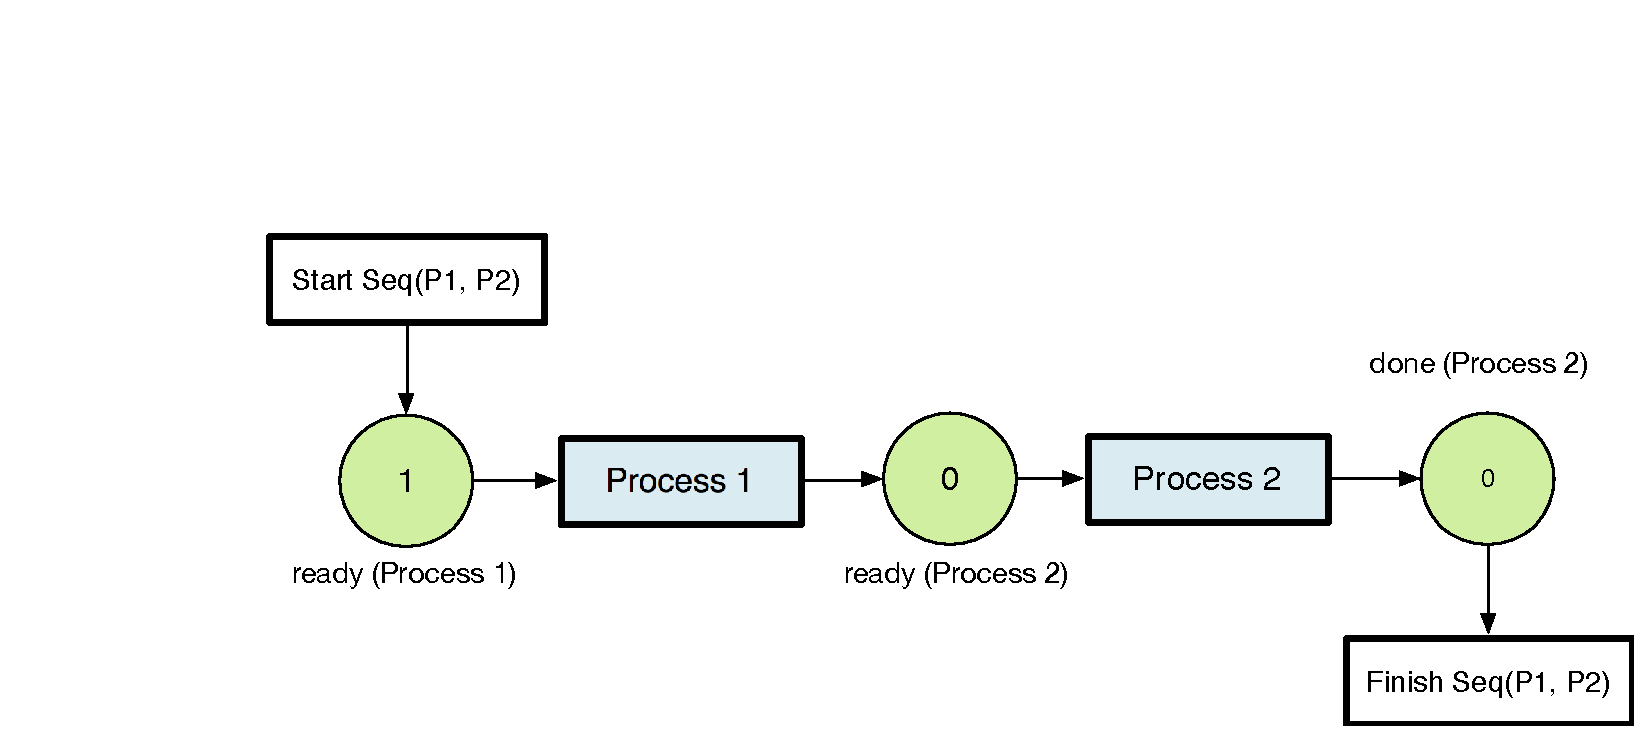
\includegraphics[width=0.9\columnwidth]{seq-simple.eps}
    \caption{The sequence construct}
    \label{fig:Conditional effects and outputs}
\end{figure}

\begin{figure}[h]
    \centering
    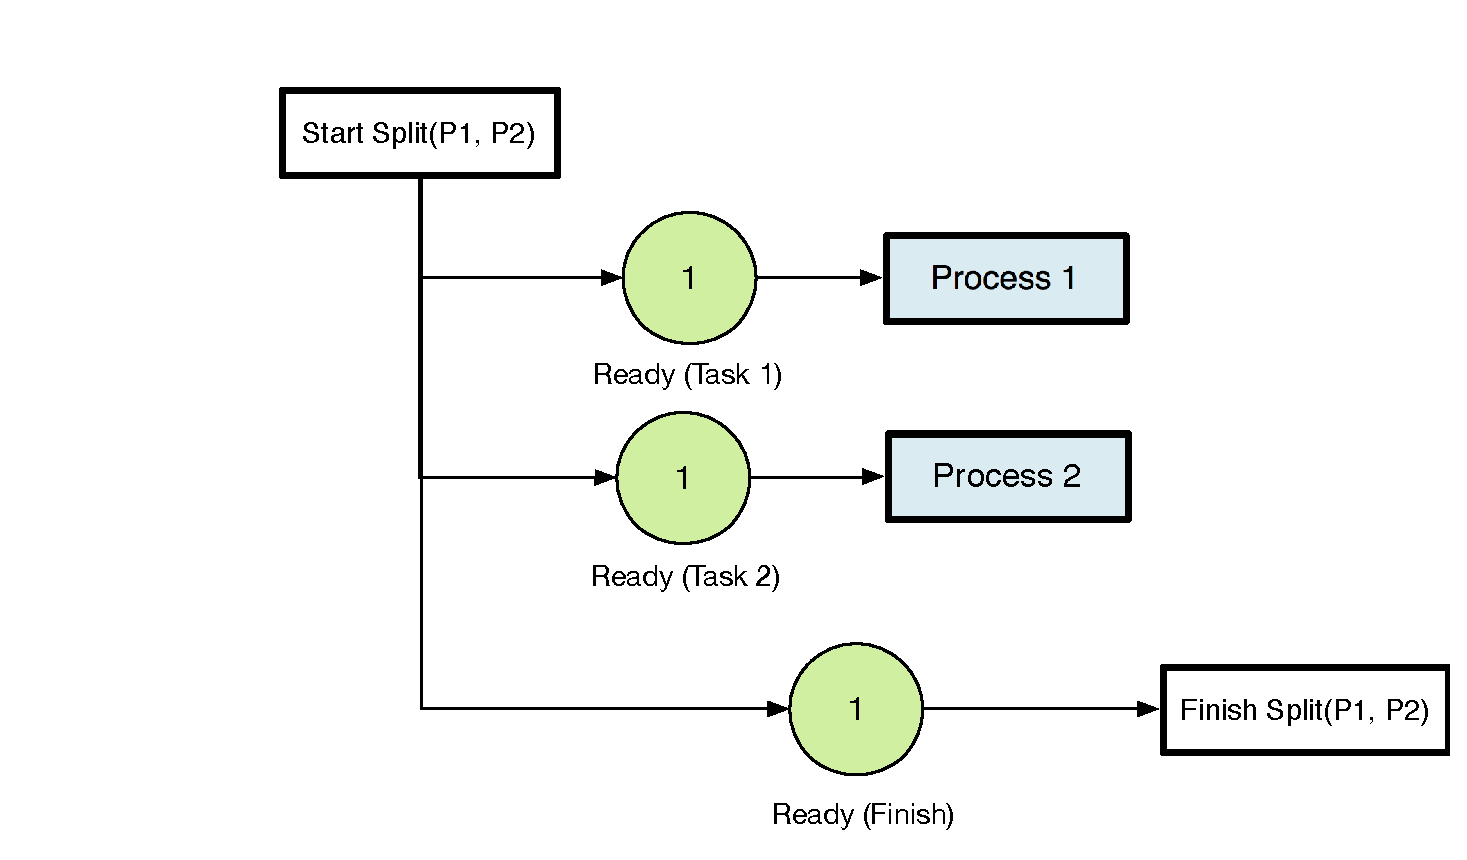
\includegraphics[width=0.9\columnwidth]{seq-split.eps}
    \caption{The sequence construct}
    \label{fig:Conditional effects and outputs}
\end{figure}

\begin{figure}[h]
    \centering
    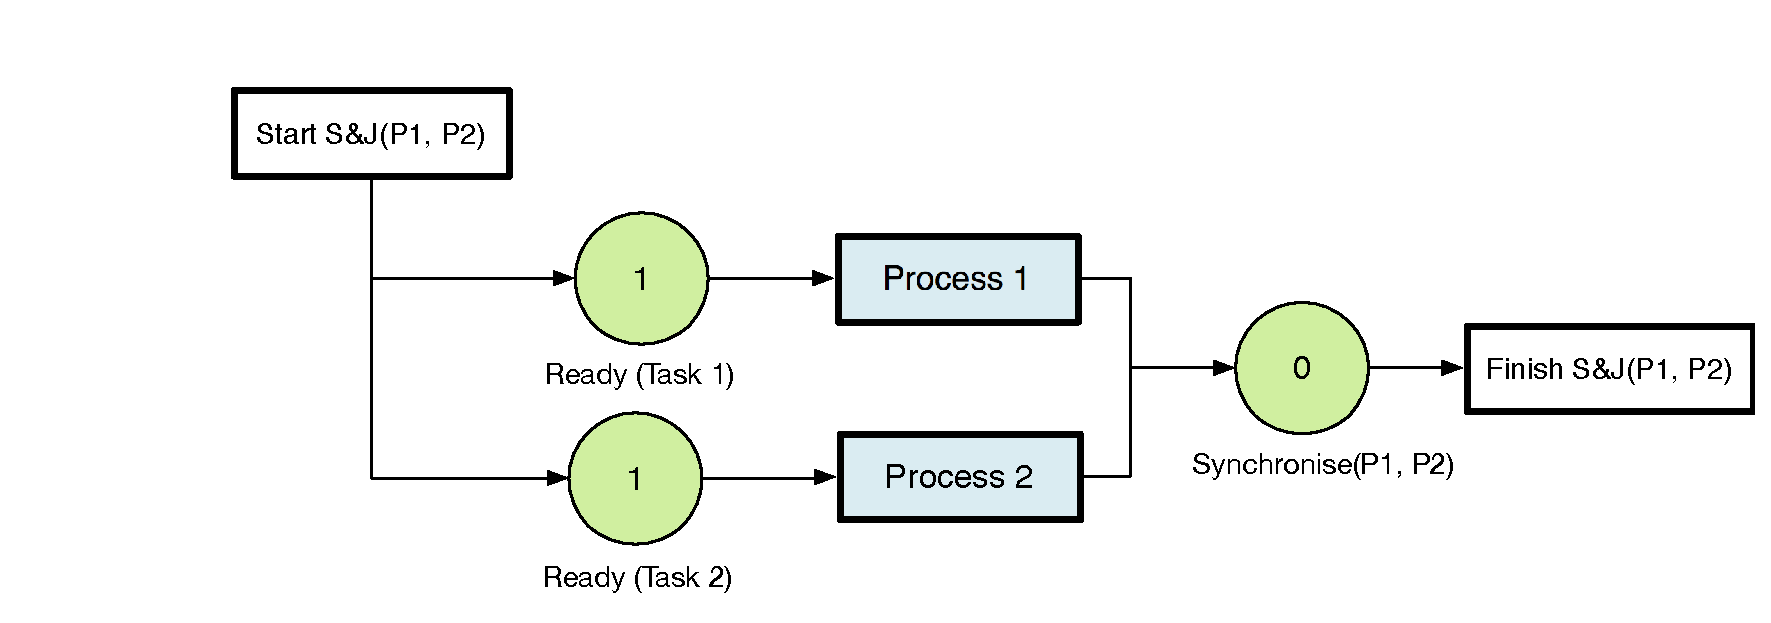
\includegraphics[width=0.9\columnwidth]{seq-split-join.eps}
    \caption{The sequence construct}
    \label{fig:Conditional effects and outputs}
\end{figure}

\begin{figure}[h]
    \centering
    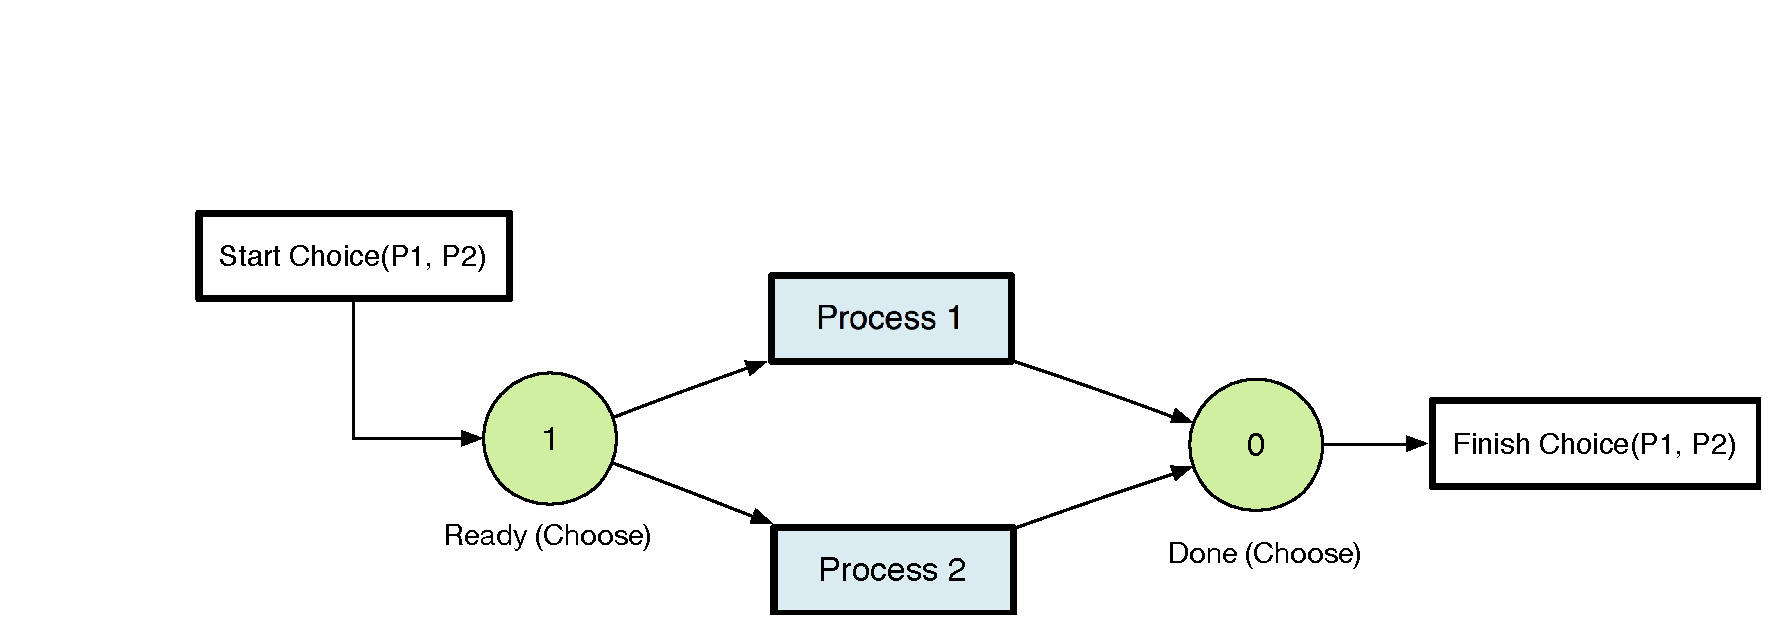
\includegraphics[width=0.9\columnwidth]{seq-choice.eps}
    \caption{The sequence construct}
    \label{fig:Conditional effects and outputs}
\end{figure}

\begin{figure}[h]
    \centering
    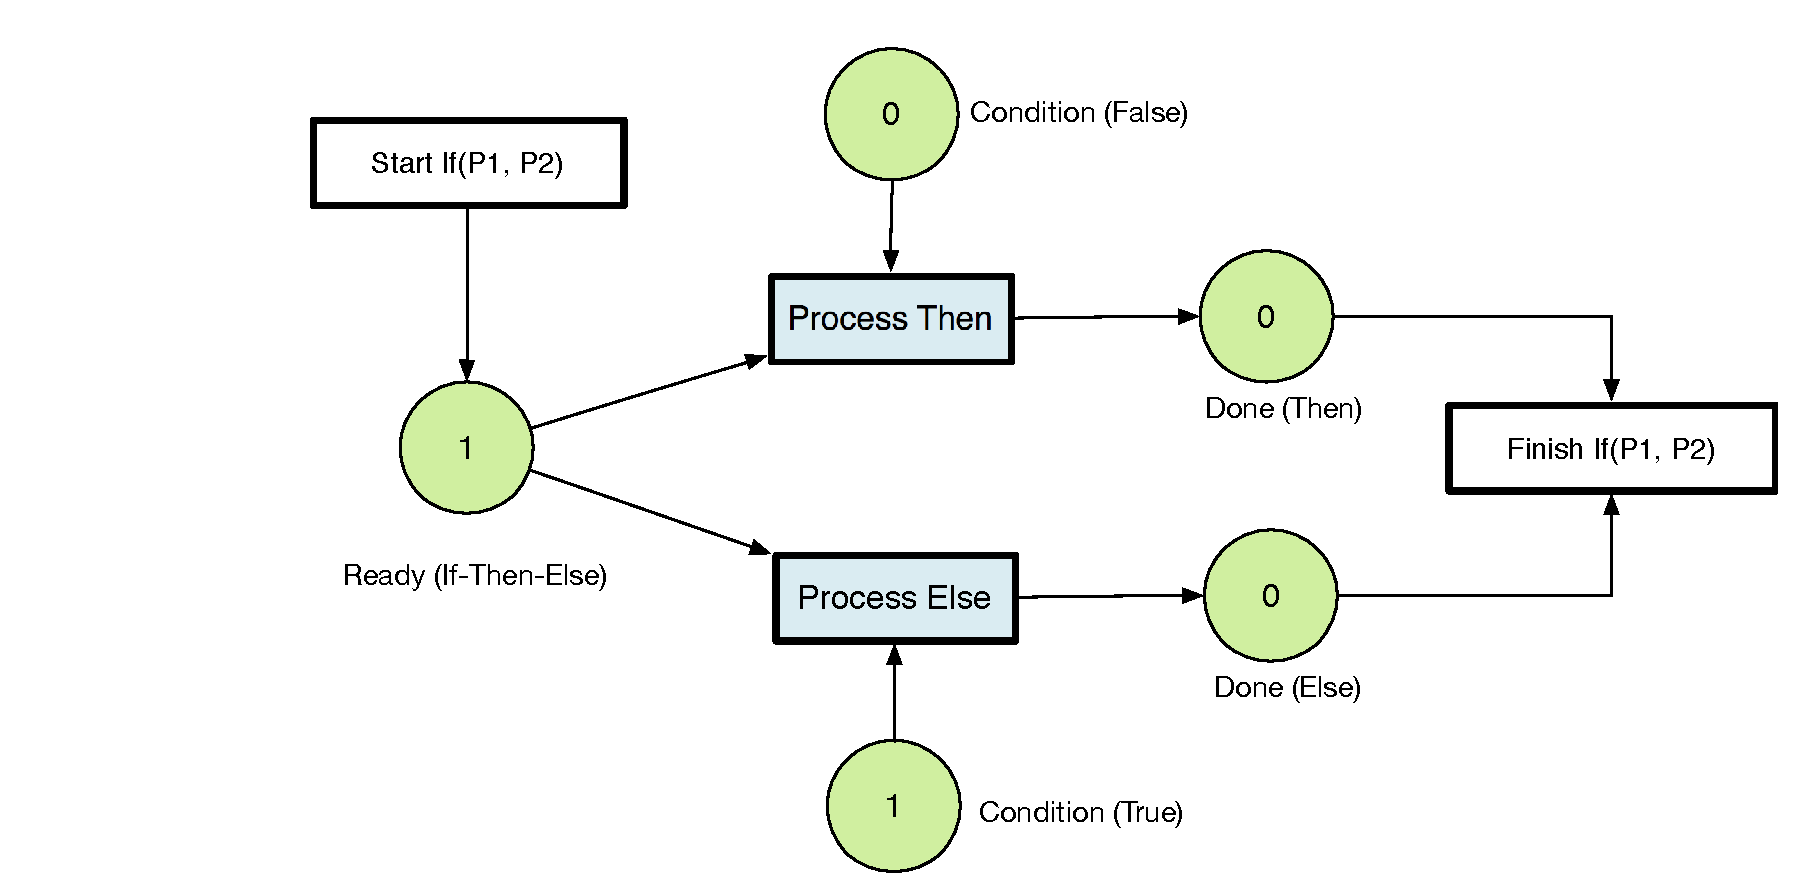
\includegraphics[width=1\columnwidth]{seq-if.eps}
    \caption{The sequence construct}
    \label{fig:Conditional effects and outputs}
\end{figure}

\begin{figure}[h]
    \centering
    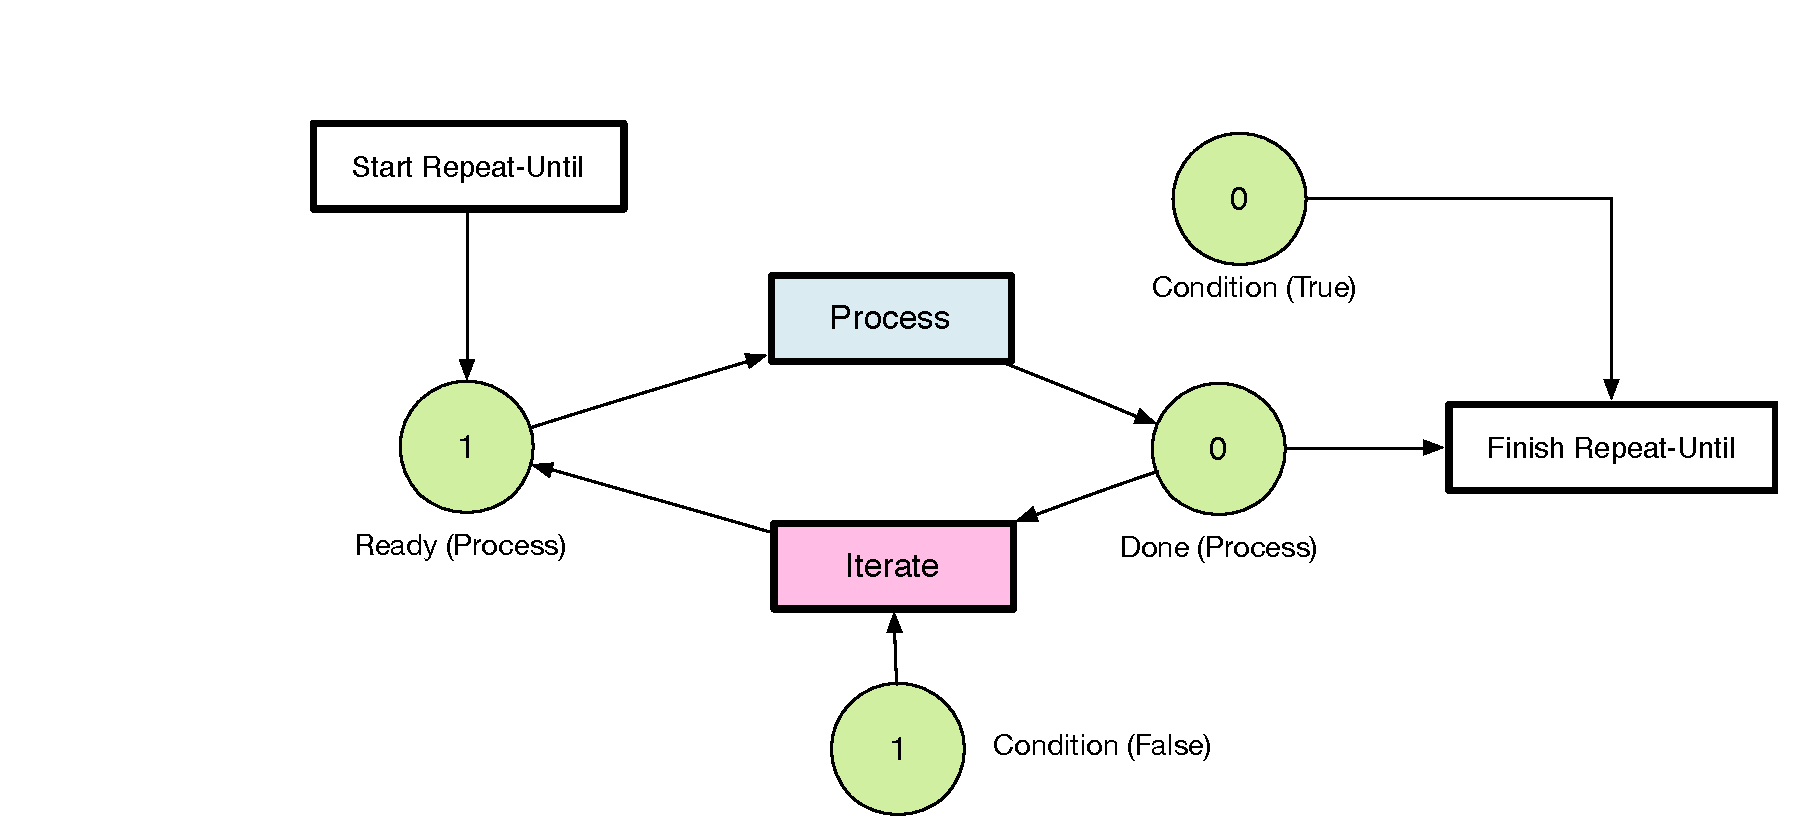
\includegraphics[width=1\columnwidth]{seq-iterate.eps}
    \caption{The sequence construct}
    \label{fig:Conditional effects and outputs}
\end{figure}